


% Header, overrides base

% Make sure that the sphinx doc style knows who it inherits from.
\def\sphinxdocclass{article}

% Declare the document class
\documentclass[letterpaper,10pt,english]{/usr/local/EPD7.3/lib/python2.7/site-packages/sphinx/texinputs/sphinxhowto}

% Imports
\usepackage[utf8]{inputenc}
\DeclareUnicodeCharacter{00A0}{\\nobreakspace}
\usepackage[T1]{fontenc}
\usepackage{babel}
\usepackage{times}
\usepackage{import}
\usepackage[Bjarne]{/usr/local/EPD7.3/lib/python2.7/site-packages/sphinx/texinputs/fncychap}
\usepackage{longtable}
\usepackage{/usr/local/EPD7.3/lib/python2.7/site-packages/sphinx/texinputs/sphinx}
\usepackage{multirow}

\usepackage{amsmath}
\usepackage{amssymb}
\usepackage{ucs}
\usepackage[]{caption}
\usepackage{filecontents}
\pagenumbering{arabic}
\pagestyle{plain}
\usepackage{enumerate}

% Used to make the Input/Output rules follow around the contents.
\usepackage{needspace}

% Pygments requirements
\usepackage{fancyvrb}
\usepackage{color}
% ansi colors additions
\definecolor{darkgreen}{rgb}{.12,.54,.11}
\definecolor{lightgray}{gray}{.95}
\definecolor{brown}{rgb}{0.54,0.27,0.07}
\definecolor{purple}{rgb}{0.5,0.0,0.5}
\definecolor{darkgray}{gray}{0.25}
\definecolor{lightred}{rgb}{1.0,0.39,0.28}
\definecolor{lightgreen}{rgb}{0.48,0.99,0.0}
\definecolor{lightblue}{rgb}{0.53,0.81,0.92}
\definecolor{lightpurple}{rgb}{0.87,0.63,0.87}
\definecolor{lightcyan}{rgb}{0.5,1.0,0.83}

% Needed to box output/input
\usepackage{tikz}
\usetikzlibrary{calc,arrows,shadows}
\usepackage[framemethod=tikz]{mdframed}

\usepackage{alltt}

% Used to load and display graphics
\usepackage{graphicx}
\graphicspath{ {figs/} }
\usepackage[Export]{adjustbox} % To resize

% used so that images for notebooks which have spaces in the name can still be included
\usepackage{grffile}


% For formatting output while also word wrapping.
\usepackage{listings}
\lstset{breaklines=true}
\lstset{basicstyle=\small\ttfamily}
\def\smaller{\fontsize{9.5pt}{9.5pt}\selectfont}

%Pygments definitions

\makeatletter
\def\PY@reset{\let\PY@it=\relax \let\PY@bf=\relax%
\let\PY@ul=\relax \let\PY@tc=\relax%
\let\PY@bc=\relax \let\PY@ff=\relax}
\def\PY@tok#1{\csname PY@tok@#1\endcsname}
\def\PY@toks#1+{\ifx\relax#1\empty\else%
\PY@tok{#1}\expandafter\PY@toks\fi}
\def\PY@do#1{\PY@bc{\PY@tc{\PY@ul{%
\PY@it{\PY@bf{\PY@ff{#1}}}}}}}
\def\PY#1#2{\PY@reset\PY@toks#1+\relax+\PY@do{#2}}

\expandafter\def\csname PY@tok@gd\endcsname{\def\PY@tc##1{\textcolor[rgb]{0.63,0.00,0.00}{##1}}}
\expandafter\def\csname PY@tok@gu\endcsname{\let\PY@bf=\textbf\def\PY@tc##1{\textcolor[rgb]{0.50,0.00,0.50}{##1}}}
\expandafter\def\csname PY@tok@gt\endcsname{\def\PY@tc##1{\textcolor[rgb]{0.00,0.27,0.87}{##1}}}
\expandafter\def\csname PY@tok@gs\endcsname{\let\PY@bf=\textbf}
\expandafter\def\csname PY@tok@gr\endcsname{\def\PY@tc##1{\textcolor[rgb]{1.00,0.00,0.00}{##1}}}
\expandafter\def\csname PY@tok@cm\endcsname{\let\PY@it=\textit\def\PY@tc##1{\textcolor[rgb]{0.25,0.50,0.50}{##1}}}
\expandafter\def\csname PY@tok@vg\endcsname{\def\PY@tc##1{\textcolor[rgb]{0.10,0.09,0.49}{##1}}}
\expandafter\def\csname PY@tok@m\endcsname{\def\PY@tc##1{\textcolor[rgb]{0.40,0.40,0.40}{##1}}}
\expandafter\def\csname PY@tok@mh\endcsname{\def\PY@tc##1{\textcolor[rgb]{0.40,0.40,0.40}{##1}}}
\expandafter\def\csname PY@tok@go\endcsname{\def\PY@tc##1{\textcolor[rgb]{0.53,0.53,0.53}{##1}}}
\expandafter\def\csname PY@tok@ge\endcsname{\let\PY@it=\textit}
\expandafter\def\csname PY@tok@vc\endcsname{\def\PY@tc##1{\textcolor[rgb]{0.10,0.09,0.49}{##1}}}
\expandafter\def\csname PY@tok@il\endcsname{\def\PY@tc##1{\textcolor[rgb]{0.40,0.40,0.40}{##1}}}
\expandafter\def\csname PY@tok@cs\endcsname{\let\PY@it=\textit\def\PY@tc##1{\textcolor[rgb]{0.25,0.50,0.50}{##1}}}
\expandafter\def\csname PY@tok@cp\endcsname{\def\PY@tc##1{\textcolor[rgb]{0.74,0.48,0.00}{##1}}}
\expandafter\def\csname PY@tok@gi\endcsname{\def\PY@tc##1{\textcolor[rgb]{0.00,0.63,0.00}{##1}}}
\expandafter\def\csname PY@tok@gh\endcsname{\let\PY@bf=\textbf\def\PY@tc##1{\textcolor[rgb]{0.00,0.00,0.50}{##1}}}
\expandafter\def\csname PY@tok@ni\endcsname{\let\PY@bf=\textbf\def\PY@tc##1{\textcolor[rgb]{0.60,0.60,0.60}{##1}}}
\expandafter\def\csname PY@tok@nl\endcsname{\def\PY@tc##1{\textcolor[rgb]{0.63,0.63,0.00}{##1}}}
\expandafter\def\csname PY@tok@nn\endcsname{\let\PY@bf=\textbf\def\PY@tc##1{\textcolor[rgb]{0.00,0.00,1.00}{##1}}}
\expandafter\def\csname PY@tok@no\endcsname{\def\PY@tc##1{\textcolor[rgb]{0.53,0.00,0.00}{##1}}}
\expandafter\def\csname PY@tok@na\endcsname{\def\PY@tc##1{\textcolor[rgb]{0.49,0.56,0.16}{##1}}}
\expandafter\def\csname PY@tok@nb\endcsname{\def\PY@tc##1{\textcolor[rgb]{0.00,0.50,0.00}{##1}}}
\expandafter\def\csname PY@tok@nc\endcsname{\let\PY@bf=\textbf\def\PY@tc##1{\textcolor[rgb]{0.00,0.00,1.00}{##1}}}
\expandafter\def\csname PY@tok@nd\endcsname{\def\PY@tc##1{\textcolor[rgb]{0.67,0.13,1.00}{##1}}}
\expandafter\def\csname PY@tok@ne\endcsname{\let\PY@bf=\textbf\def\PY@tc##1{\textcolor[rgb]{0.82,0.25,0.23}{##1}}}
\expandafter\def\csname PY@tok@nf\endcsname{\def\PY@tc##1{\textcolor[rgb]{0.00,0.00,1.00}{##1}}}
\expandafter\def\csname PY@tok@si\endcsname{\let\PY@bf=\textbf\def\PY@tc##1{\textcolor[rgb]{0.73,0.40,0.53}{##1}}}
\expandafter\def\csname PY@tok@s2\endcsname{\def\PY@tc##1{\textcolor[rgb]{0.73,0.13,0.13}{##1}}}
\expandafter\def\csname PY@tok@vi\endcsname{\def\PY@tc##1{\textcolor[rgb]{0.10,0.09,0.49}{##1}}}
\expandafter\def\csname PY@tok@nt\endcsname{\let\PY@bf=\textbf\def\PY@tc##1{\textcolor[rgb]{0.00,0.50,0.00}{##1}}}
\expandafter\def\csname PY@tok@nv\endcsname{\def\PY@tc##1{\textcolor[rgb]{0.10,0.09,0.49}{##1}}}
\expandafter\def\csname PY@tok@s1\endcsname{\def\PY@tc##1{\textcolor[rgb]{0.73,0.13,0.13}{##1}}}
\expandafter\def\csname PY@tok@sh\endcsname{\def\PY@tc##1{\textcolor[rgb]{0.73,0.13,0.13}{##1}}}
\expandafter\def\csname PY@tok@sc\endcsname{\def\PY@tc##1{\textcolor[rgb]{0.73,0.13,0.13}{##1}}}
\expandafter\def\csname PY@tok@sx\endcsname{\def\PY@tc##1{\textcolor[rgb]{0.00,0.50,0.00}{##1}}}
\expandafter\def\csname PY@tok@bp\endcsname{\def\PY@tc##1{\textcolor[rgb]{0.00,0.50,0.00}{##1}}}
\expandafter\def\csname PY@tok@c1\endcsname{\let\PY@it=\textit\def\PY@tc##1{\textcolor[rgb]{0.25,0.50,0.50}{##1}}}
\expandafter\def\csname PY@tok@kc\endcsname{\let\PY@bf=\textbf\def\PY@tc##1{\textcolor[rgb]{0.00,0.50,0.00}{##1}}}
\expandafter\def\csname PY@tok@c\endcsname{\let\PY@it=\textit\def\PY@tc##1{\textcolor[rgb]{0.25,0.50,0.50}{##1}}}
\expandafter\def\csname PY@tok@mf\endcsname{\def\PY@tc##1{\textcolor[rgb]{0.40,0.40,0.40}{##1}}}
\expandafter\def\csname PY@tok@err\endcsname{\def\PY@bc##1{\setlength{\fboxsep}{0pt}\fcolorbox[rgb]{1.00,0.00,0.00}{1,1,1}{\strut ##1}}}
\expandafter\def\csname PY@tok@kd\endcsname{\let\PY@bf=\textbf\def\PY@tc##1{\textcolor[rgb]{0.00,0.50,0.00}{##1}}}
\expandafter\def\csname PY@tok@ss\endcsname{\def\PY@tc##1{\textcolor[rgb]{0.10,0.09,0.49}{##1}}}
\expandafter\def\csname PY@tok@sr\endcsname{\def\PY@tc##1{\textcolor[rgb]{0.73,0.40,0.53}{##1}}}
\expandafter\def\csname PY@tok@mo\endcsname{\def\PY@tc##1{\textcolor[rgb]{0.40,0.40,0.40}{##1}}}
\expandafter\def\csname PY@tok@kn\endcsname{\let\PY@bf=\textbf\def\PY@tc##1{\textcolor[rgb]{0.00,0.50,0.00}{##1}}}
\expandafter\def\csname PY@tok@mi\endcsname{\def\PY@tc##1{\textcolor[rgb]{0.40,0.40,0.40}{##1}}}
\expandafter\def\csname PY@tok@gp\endcsname{\let\PY@bf=\textbf\def\PY@tc##1{\textcolor[rgb]{0.00,0.00,0.50}{##1}}}
\expandafter\def\csname PY@tok@o\endcsname{\def\PY@tc##1{\textcolor[rgb]{0.40,0.40,0.40}{##1}}}
\expandafter\def\csname PY@tok@kr\endcsname{\let\PY@bf=\textbf\def\PY@tc##1{\textcolor[rgb]{0.00,0.50,0.00}{##1}}}
\expandafter\def\csname PY@tok@s\endcsname{\def\PY@tc##1{\textcolor[rgb]{0.73,0.13,0.13}{##1}}}
\expandafter\def\csname PY@tok@kp\endcsname{\def\PY@tc##1{\textcolor[rgb]{0.00,0.50,0.00}{##1}}}
\expandafter\def\csname PY@tok@w\endcsname{\def\PY@tc##1{\textcolor[rgb]{0.73,0.73,0.73}{##1}}}
\expandafter\def\csname PY@tok@kt\endcsname{\def\PY@tc##1{\textcolor[rgb]{0.69,0.00,0.25}{##1}}}
\expandafter\def\csname PY@tok@ow\endcsname{\let\PY@bf=\textbf\def\PY@tc##1{\textcolor[rgb]{0.67,0.13,1.00}{##1}}}
\expandafter\def\csname PY@tok@sb\endcsname{\def\PY@tc##1{\textcolor[rgb]{0.73,0.13,0.13}{##1}}}
\expandafter\def\csname PY@tok@k\endcsname{\let\PY@bf=\textbf\def\PY@tc##1{\textcolor[rgb]{0.00,0.50,0.00}{##1}}}
\expandafter\def\csname PY@tok@se\endcsname{\let\PY@bf=\textbf\def\PY@tc##1{\textcolor[rgb]{0.73,0.40,0.13}{##1}}}
\expandafter\def\csname PY@tok@sd\endcsname{\let\PY@it=\textit\def\PY@tc##1{\textcolor[rgb]{0.73,0.13,0.13}{##1}}}

\def\PYZbs{\char`\\}
\def\PYZus{\char`\_}
\def\PYZob{\char`\{}
\def\PYZcb{\char`\}}
\def\PYZca{\char`\^}
\def\PYZam{\char`\&}
\def\PYZlt{\char`\<}
\def\PYZgt{\char`\>}
\def\PYZsh{\char`\#}
\def\PYZpc{\char`\%}
\def\PYZdl{\char`\$}
\def\PYZhy{\char`\-}
\def\PYZsq{\char`\'}
\def\PYZdq{\char`\"}
\def\PYZti{\char`\~}
% for compatibility with earlier versions
\def\PYZat{@}
\def\PYZlb{[}
\def\PYZrb{]}
\makeatother


%Set pygments styles if needed...

\definecolor{nbframe-border}{rgb}{0.867,0.867,0.867}
\definecolor{nbframe-bg}{rgb}{0.969,0.969,0.969}
\definecolor{nbframe-in-prompt}{rgb}{0.0,0.0,0.502}
\definecolor{nbframe-out-prompt}{rgb}{0.545,0.0,0.0}

\newenvironment{ColorVerbatim}
{\begin{mdframed}[%
roundcorner=1.0pt, %
backgroundcolor=nbframe-bg, %
userdefinedwidth=1\linewidth, %
leftmargin=0.1\linewidth, %
innerleftmargin=0pt, %
innerrightmargin=0pt, %
linecolor=nbframe-border, %
linewidth=1pt, %
usetwoside=false, %
everyline=true, %
innerlinewidth=3pt, %
innerlinecolor=nbframe-bg, %
middlelinewidth=1pt, %
middlelinecolor=nbframe-bg, %
outerlinewidth=0.5pt, %
outerlinecolor=nbframe-border, %
needspace=0pt
]}
{\end{mdframed}}

\newenvironment{InvisibleVerbatim}
{\begin{mdframed}[leftmargin=0.1\linewidth,innerleftmargin=3pt,innerrightmargin=3pt, userdefinedwidth=1\linewidth, linewidth=0pt, linecolor=white, usetwoside=false]}
{\end{mdframed}}

\renewenvironment{Verbatim}[1][\unskip]
{\begin{alltt}\smaller}
{\end{alltt}}


% Help prevent overflowing lines due to urls and other hard-to-break
% entities.  This doesn't catch everything...
\sloppy

% Document level variables
\title{Basic Operations of PyParty}\footnotetext[1]{{George Washington University; Dept. of Physics; Condensed Matter Group (PI: Mark Reeves- reevesme@gwu.edu).  Content claim excludes all references to to open source software, including iPython and its corresponding notebook and nbconvert utilities.  Please direct inquiries to Adam Hughes (hugadams@gwmail.gwu.edu)}}
\date{December 12, 2013}
\release{}
\author{Adam Hughes}
\renewcommand{\releasename}{}

% TODO: Add option for the user to specify a logo for his/her export.
\newcommand{\sphinxlogo}{}

% Make the index page of the document.
\makeindex

% Import sphinx document type specifics.



% Body

% Start of the document
\begin{document}
\begin{figure}[h!]\centering
\caption*{\scriptsize \color{red} \copyright \; Original content herein is the intellectual property of the GWU Cond. Matter Group\footnotemark{}}
\includegraphics[width=8cm]{/usr/local/bin/gwulogo}
\end{figure}


\maketitle 
 \tableofcontents
\newpage






\subsection{Imports/configuration
}

% Make sure that atleast 4 lines are below the HR
\needspace{4\baselineskip}


\vspace{6pt}
\makebox[0.1\linewidth]{\smaller\hfill\tt\color{nbframe-in-prompt}In\hspace{4pt}{[}17{]}:\hspace{4pt}}\\*
\vspace{-2.65\baselineskip}
\begin{ColorVerbatim}
\vspace{-0.7\baselineskip}
\begin{Verbatim}[commandchars=\\\{\}]
\PY{n}{pylabl}\PY{o}{.}\PY{n}{rcParams}\PY{p}{[}\PY{l+s}{\PYZsq{}}\PY{l+s}{figure.figsize}\PY{l+s}{\PYZsq{}}\PY{p}{]} \PY{o}{=} \PY{l+m+mi}{8}\PY{p}{,} \PY{l+m+mf}{5.5}
\PY{k+kn}{import} \PY{n+nn}{numpy} \PY{k+kn}{as} \PY{n+nn}{np}
\end{Verbatim}


\vspace{-0.2\baselineskip}

\end{ColorVerbatim}

\part{PyParty Tutorial
}\section{The Canvas Class
}\emph{Canvas} is the primary object that users will deal with in
the pre-alpha version of pyparty. The canvas itself is a composite
class, storing both an image (numpy.ndarray : \emph{.image}) and a
custom container for storing and manipulating particles
(pyparty.ParticleManager : \emph{.particles}).

To create a canvas, which is an image (ndarray) and a special
container (ParticleManager) that stores, tracks and draws particles
into the image (via array indexing).


% Make sure that atleast 4 lines are below the HR
\needspace{4\baselineskip}


\vspace{6pt}
\makebox[0.1\linewidth]{\smaller\hfill\tt\color{nbframe-in-prompt}In\hspace{4pt}{[}18{]}:\hspace{4pt}}\\*
\vspace{-2.65\baselineskip}
\begin{ColorVerbatim}
\vspace{-0.7\baselineskip}
\begin{Verbatim}[commandchars=\\\{\}]
\PY{k+kn}{from} \PY{n+nn}{pyparty.tools.canvas} \PY{k+kn}{import} \PY{n}{Canvas}

\PY{n}{c}\PY{o}{=}\PY{n}{Canvas}\PY{p}{(}\PY{p}{)}
\PY{k}{print} \PY{p}{(}\PY{n+nb}{type}\PY{p}{(}\PY{n}{c}\PY{p}{)}\PY{p}{,} \PY{n+nb}{type}\PY{p}{(}\PY{n}{c}\PY{o}{.}\PY{n}{image}\PY{p}{)}\PY{p}{,} \PY{n+nb}{type}\PY{p}{(}\PY{n}{c}\PY{o}{.}\PY{n}{\PYZus{}particles}\PY{p}{)}\PY{p}{)}
\end{Verbatim}


\vspace{-0.2\baselineskip}

\end{ColorVerbatim}




% If the first block is an image, minipage the image.  Else
% request a certain amount of space for the input text.
\needspace{4\baselineskip}



% Add document contents.

\begin{InvisibleVerbatim}
\vspace{-0.5\baselineskip}
\begin{alltt}(<class 'pyparty.tools.canvas.Canvas'>, <type 'numpy.ndarray'>, <class
'pyparty.tools.manager.ParticleManager'>)
\end{alltt}

\end{InvisibleVerbatim}



The canvas tries to acts as an intuitive hybrid object for an image
with particles, and selectives promotes the API of both images. For
example, the public attribute \emph{particles} hides the underlying
\emph{ParticleManager} instance, and instead returns particles as a
list of tuples.


% Make sure that atleast 4 lines are below the HR
\needspace{4\baselineskip}


\vspace{6pt}
\makebox[0.1\linewidth]{\smaller\hfill\tt\color{nbframe-in-prompt}In\hspace{4pt}{[}19{]}:\hspace{4pt}}\\*
\vspace{-2.65\baselineskip}
\begin{ColorVerbatim}
\vspace{-0.7\baselineskip}
\begin{Verbatim}[commandchars=\\\{\}]
\PY{k}{print} \PY{n+nb}{type}\PY{p}{(}\PY{n}{c}\PY{o}{.}\PY{n}{image}\PY{p}{)}\PY{p}{,} \PY{n+nb}{type}\PY{p}{(}\PY{n}{c}\PY{o}{.}\PY{n}{particles}\PY{p}{)}
\end{Verbatim}


\vspace{-0.2\baselineskip}

\end{ColorVerbatim}




% If the first block is an image, minipage the image.  Else
% request a certain amount of space for the input text.
\needspace{4\baselineskip}



% Add document contents.

\begin{InvisibleVerbatim}
\vspace{-0.5\baselineskip}
\begin{alltt}<type 'numpy.ndarray'> <type 'list'>
\end{alltt}

\end{InvisibleVerbatim}



The reason that \emph{\_particles} is a private method is because
Canvas promotes its own ParticleManager api through
\emph{particles}, which be default, returns a list of particle
names (see next section). Since canvas is a composite class between
an ndarray and Particle manager, I decided that attribute lookup
should defer to the image (eg):


% Make sure that atleast 4 lines are below the HR
\needspace{4\baselineskip}


\vspace{6pt}
\makebox[0.1\linewidth]{\smaller\hfill\tt\color{nbframe-in-prompt}In\hspace{4pt}{[}20{]}:\hspace{4pt}}\\*
\vspace{-2.65\baselineskip}
\begin{ColorVerbatim}
\vspace{-0.7\baselineskip}
\begin{Verbatim}[commandchars=\\\{\}]
\PY{k}{print} \PY{n}{c}\PY{o}{.}\PY{n}{image}\PY{o}{.}\PY{n}{shape}
\PY{k}{print} \PY{n}{c}\PY{o}{.}\PY{n}{shape} \PY{c}{\PYZsh{}}
\end{Verbatim}


\vspace{-0.2\baselineskip}

\end{ColorVerbatim}




% If the first block is an image, minipage the image.  Else
% request a certain amount of space for the input text.
\needspace{4\baselineskip}



% Add document contents.

\begin{InvisibleVerbatim}
\vspace{-0.5\baselineskip}
\begin{alltt}(512, 512, 3)
(512, 512, 3)
\end{alltt}

\end{InvisibleVerbatim}



While slicing/indexing (see below) should defer to the particles,
as the user could easily manipulate the image before and after
applying particles.
\section{Adding particles
}Particles can be added to an image in a variety of ways.
\subsection{Manually by passing parameters
}First let's see what available particle types there are:


% Make sure that atleast 4 lines are below the HR
\needspace{4\baselineskip}


\vspace{6pt}
\makebox[0.1\linewidth]{\smaller\hfill\tt\color{nbframe-in-prompt}In\hspace{4pt}{[}21{]}:\hspace{4pt}}\\*
\vspace{-2.65\baselineskip}
\begin{ColorVerbatim}
\vspace{-0.7\baselineskip}
\begin{Verbatim}[commandchars=\\\{\}]
\PY{n}{c}\PY{o}{.}\PY{n}{\PYZus{}particles}\PY{o}{.}\PY{n}{available}\PY{p}{(}\PY{p}{)}
\end{Verbatim}


\vspace{-0.2\baselineskip}

\end{ColorVerbatim}




% If the first block is an image, minipage the image.  Else
% request a certain amount of space for the input text.
\needspace{4\baselineskip}



% Add document contents.

\makebox[0.1\linewidth]{\smaller\hfill\tt\color{nbframe-out-prompt}Out\hspace{4pt}{[}21{]}:\hspace{4pt}}\\*
\vspace{-2.55\baselineskip}\begin{InvisibleVerbatim}
\vspace{-0.5\baselineskip}
\begin{alltt}('circle', 'dimer')\end{alltt}

\end{InvisibleVerbatim}





% Make sure that atleast 4 lines are below the HR
\needspace{4\baselineskip}


\vspace{6pt}
\makebox[0.1\linewidth]{\smaller\hfill\tt\color{nbframe-in-prompt}In\hspace{4pt}{[}22{]}:\hspace{4pt}}\\*
\vspace{-2.65\baselineskip}
\begin{ColorVerbatim}
\vspace{-0.7\baselineskip}
\begin{Verbatim}[commandchars=\\\{\}]
\PY{n}{c}\PY{o}{.}\PY{n}{add}\PY{p}{(}\PY{l+s}{\PYZsq{}}\PY{l+s}{circle}\PY{l+s}{\PYZsq{}}\PY{p}{,} \PY{n}{name}\PY{o}{=}\PY{l+s}{\PYZsq{}}\PY{l+s}{centered\PYZus{}particle}\PY{l+s}{\PYZsq{}}\PY{p}{,} \PY{n}{radius}\PY{o}{=}\PY{l+m+mi}{20}\PY{p}{,} \PY{n}{center}\PY{o}{=}\PY{p}{(}\PY{l+m+mi}{255}\PY{p}{,}\PY{l+m+mi}{256}\PY{p}{)}\PY{p}{,} \PY{n}{color}\PY{o}{=}\PY{p}{(}\PY{l+m+mi}{0}\PY{p}{,}\PY{o}{.}\PY{l+m+mi}{1}\PY{p}{,}\PY{o}{.}\PY{l+m+mi}{5}\PY{p}{)}\PY{p}{)}
\PY{n}{c}\PY{o}{.}\PY{n}{add}\PY{p}{(}\PY{l+s}{\PYZsq{}}\PY{l+s}{circle}\PY{l+s}{\PYZsq{}}\PY{p}{,} \PY{n}{name}\PY{o}{=}\PY{l+s}{\PYZsq{}}\PY{l+s}{edge\PYZus{}particle}\PY{l+s}{\PYZsq{}}\PY{p}{,} \PY{n}{radius}\PY{o}{=}\PY{l+m+mi}{100}\PY{p}{,} \PY{n}{center}\PY{o}{=}\PY{p}{(}\PY{l+m+mi}{0}\PY{p}{,}\PY{l+m+mi}{0}\PY{p}{)}\PY{p}{,} \PY{n}{color}\PY{o}{=}\PY{p}{(}\PY{l+m+mi}{0}\PY{p}{,}\PY{l+m+mi}{1}\PY{p}{,}\PY{l+m+mi}{0}\PY{p}{)}\PY{p}{,} \PY{n}{shape}\PY{o}{=}\PY{n}{c}\PY{o}{.}\PY{n}{image}\PY{o}{.}\PY{n}{shape}\PY{p}{)}
\PY{n}{c}\PY{o}{.}\PY{n}{add}\PY{p}{(}\PY{l+s}{\PYZsq{}}\PY{l+s}{circle}\PY{l+s}{\PYZsq{}}\PY{p}{,} \PY{n}{name}\PY{o}{=}\PY{l+s}{\PYZsq{}}\PY{l+s}{outside\PYZus{}particle}\PY{l+s}{\PYZsq{}}\PY{p}{,} \PY{n}{radius}\PY{o}{=}\PY{l+m+mi}{20}\PY{p}{,} \PY{n}{center}\PY{o}{=}\PY{p}{(}\PY{l+m+mi}{900}\PY{p}{,}\PY{l+m+mi}{200}\PY{p}{)}\PY{p}{,} \PY{n}{color}\PY{o}{=}\PY{p}{(}\PY{l+m+mi}{0}\PY{p}{,}\PY{o}{.}\PY{l+m+mi}{1}\PY{p}{,}\PY{o}{.}\PY{l+m+mi}{5}\PY{p}{)}\PY{p}{)}

\PY{n}{named} \PY{o}{=} \PY{n}{c}\PY{o}{.}\PY{n}{particles}
\PY{n}{named}
\end{Verbatim}


\vspace{-0.2\baselineskip}

\end{ColorVerbatim}




% If the first block is an image, minipage the image.  Else
% request a certain amount of space for the input text.
\needspace{4\baselineskip}



% Add document contents.

\makebox[0.1\linewidth]{\smaller\hfill\tt\color{nbframe-out-prompt}Out\hspace{4pt}{[}22{]}:\hspace{4pt}}\\*
\vspace{-2.55\baselineskip}\begin{InvisibleVerbatim}
\vspace{-0.5\baselineskip}
\begin{alltt}['centered\_particle', 'edge\_particle', 'outside\_particle']\end{alltt}

\end{InvisibleVerbatim}



If we don't provide a name, they are automatically generated of the
form (shape\_index):


% Make sure that atleast 4 lines are below the HR
\needspace{4\baselineskip}


\vspace{6pt}
\makebox[0.1\linewidth]{\smaller\hfill\tt\color{nbframe-in-prompt}In\hspace{4pt}{[}23{]}:\hspace{4pt}}\\*
\vspace{-2.65\baselineskip}
\begin{ColorVerbatim}
\vspace{-0.7\baselineskip}
\begin{Verbatim}[commandchars=\\\{\}]
\PY{k}{for} \PY{n}{idx}\PY{p}{,} \PY{n}{r} \PY{o+ow}{in} \PY{n+nb}{enumerate}\PY{p}{(} \PY{p}{(}\PY{l+m+mi}{10}\PY{p}{,} \PY{l+m+mi}{20}\PY{p}{,} \PY{l+m+mi}{30}\PY{p}{)} \PY{p}{)}\PY{p}{:}
\PY{n}{c}\PY{o}{.}\PY{n}{add}\PY{p}{(}\PY{l+s}{\PYZsq{}}\PY{l+s}{circle}\PY{l+s}{\PYZsq{}}\PY{p}{,} \PY{n}{radius}\PY{o}{=}\PY{n}{r}\PY{p}{,} \PY{n}{center}\PY{o}{=}\PY{p}{(}\PY{l+m+mi}{150}\PY{p}{,} \PY{l+m+mi}{100}\PY{o}{*}\PY{p}{(}\PY{n}{idx}\PY{o}{+}\PY{l+m+mi}{1}\PY{p}{)}\PY{p}{)}\PY{p}{,} \PY{n}{color}\PY{o}{=}\PY{p}{(}\PY{l+m+mi}{1}\PY{p}{,} \PY{l+m+mi}{0}\PY{p}{,} \PY{l+m+mi}{0}\PY{p}{)}\PY{p}{)}

\PY{n}{auto\PYZus{}named} \PY{o}{=} \PY{p}{[}\PY{n}{p} \PY{k}{for} \PY{n}{p} \PY{o+ow}{in} \PY{n}{c}\PY{o}{.}\PY{n}{particles} \PY{k}{if} \PY{n}{p} \PY{o+ow}{not} \PY{o+ow}{in} \PY{n}{named}\PY{p}{]}
\PY{n}{auto\PYZus{}named}
\end{Verbatim}


\vspace{-0.2\baselineskip}

\end{ColorVerbatim}




% If the first block is an image, minipage the image.  Else
% request a certain amount of space for the input text.
\needspace{4\baselineskip}



% Add document contents.

\makebox[0.1\linewidth]{\smaller\hfill\tt\color{nbframe-out-prompt}Out\hspace{4pt}{[}23{]}:\hspace{4pt}}\\*
\vspace{-2.55\baselineskip}\begin{InvisibleVerbatim}
\vspace{-0.5\baselineskip}
\begin{alltt}['circle\_4', 'circle\_3', 'circle\_5']\end{alltt}

\end{InvisibleVerbatim}



At any point, the image with drawn particles can be visualized with
\emph{show()}, a wrapper to \emph{matplotlib.plt.imshow()}


% Make sure that atleast 4 lines are below the HR
\needspace{4\baselineskip}


\vspace{6pt}
\makebox[0.1\linewidth]{\smaller\hfill\tt\color{nbframe-in-prompt}In\hspace{4pt}{[}24{]}:\hspace{4pt}}\\*
\vspace{-2.65\baselineskip}
\begin{ColorVerbatim}
\vspace{-0.7\baselineskip}
\begin{Verbatim}[commandchars=\\\{\}]
\PY{n}{c}\PY{o}{.}\PY{n}{show}\PY{p}{(}\PY{p}{)}\PY{p}{;}
\end{Verbatim}


\vspace{-0.2\baselineskip}

\end{ColorVerbatim}




% If the first block is an image, minipage the image.  Else
% request a certain amount of space for the input text.
\needspace{4\baselineskip}



% Add document contents.

\begin{InvisibleVerbatim}
\vspace{-0.5\baselineskip}
\begin{center}
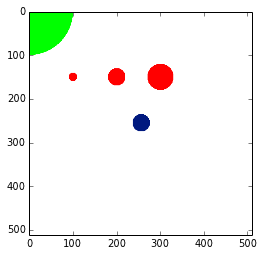
\includegraphics[max size={\textwidth}{\textheight}]{basictests_files/basictests_20_0.png}
\par
\end{center}

\end{InvisibleVerbatim}



Notice that the large circles wrap around the corners. This is
automatically done when image[rr, cc, :] is called\ldots{}
\section{Background images
}The default background is a (1024 x 768 X 3) rgb array set to
white. This was used implicitly above. We can actually pass any
array (ie image) and the particles will be redrawn over it. In the
next cell, we'll load an image from skimage's pre-packaged data.


% Make sure that atleast 4 lines are below the HR
\needspace{4\baselineskip}


\vspace{6pt}
\makebox[0.1\linewidth]{\smaller\hfill\tt\color{nbframe-in-prompt}In\hspace{4pt}{[}25{]}:\hspace{4pt}}\\*
\vspace{-2.65\baselineskip}
\begin{ColorVerbatim}
\vspace{-0.7\baselineskip}
\begin{Verbatim}[commandchars=\\\{\}]
\PY{k+kn}{from} \PY{n+nn}{skimage.data} \PY{k+kn}{import} \PY{n}{moon}

\PY{n}{c}\PY{o}{.}\PY{n}{background} \PY{o}{=} \PY{n}{moon}\PY{p}{(}\PY{p}{)}
\PY{n}{c}\PY{o}{.}\PY{n}{show}\PY{p}{(}\PY{p}{)}\PY{p}{;}
\end{Verbatim}


\vspace{-0.2\baselineskip}

\end{ColorVerbatim}




% If the first block is an image, minipage the image.  Else
% request a certain amount of space for the input text.
\needspace{4\baselineskip}



% Add document contents.

\begin{InvisibleVerbatim}
\vspace{-0.5\baselineskip}
\begin{alltt}12-12 22:16:07 WARNING  pyparty.tools.canvas:  background color has
been converted (from grayscale to RGB)
\end{alltt}

\end{InvisibleVerbatim}

\begin{InvisibleVerbatim}
\vspace{-0.5\baselineskip}
\begin{center}
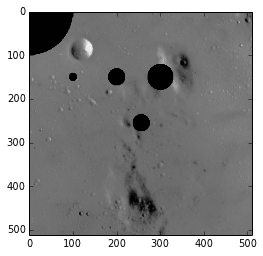
\includegraphics[max size={\textwidth}{\textheight}]{basictests_files/basictests_24_1.png}
\par
\end{center}

\end{InvisibleVerbatim}



\subsection{Image from harddrive/higher-resolution image:
}Relative or absolute paths should be automatically detected. The
image is returned by \emph{load\_background()}.


% Make sure that atleast 4 lines are below the HR
\needspace{4\baselineskip}


\vspace{6pt}
\makebox[0.1\linewidth]{\smaller\hfill\tt\color{nbframe-in-prompt}In\hspace{4pt}{[}26{]}:\hspace{4pt}}\\*
\vspace{-2.65\baselineskip}
\begin{ColorVerbatim}
\vspace{-0.7\baselineskip}
\begin{Verbatim}[commandchars=\\\{\}]
\PY{n}{tip} \PY{o}{=} \PY{n}{c}\PY{o}{.}\PY{n}{load\PYZus{}background}\PY{p}{(}\PY{l+s}{\PYZsq{}}\PY{l+s}{\PYZti{}/Desktop/brokenphone.jpg}\PY{l+s}{\PYZsq{}}\PY{p}{)} \PY{c}{\PYZsh{}Thanks Sprint...}
\PY{n}{c}\PY{o}{.}\PY{n}{show}\PY{p}{(}\PY{p}{)}
\PY{k}{print} \PY{l+s}{\PYZsq{}}\PY{l+s}{newshape = }\PY{l+s}{\PYZsq{}}\PY{p}{,} \PY{n}{c}\PY{o}{.}\PY{n}{shape}
\end{Verbatim}


\vspace{-0.2\baselineskip}

\end{ColorVerbatim}




% If the first block is an image, minipage the image.  Else
% request a certain amount of space for the input text.
\needspace{4\baselineskip}



% Add document contents.

\begin{InvisibleVerbatim}
\vspace{-0.5\baselineskip}
\begin{alltt}newshape =  (835, 626, 3)
\end{alltt}

\end{InvisibleVerbatim}

\begin{InvisibleVerbatim}
\vspace{-0.5\baselineskip}
\begin{center}
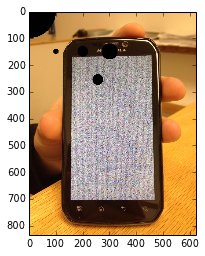
\includegraphics[max size={\textwidth}{\textheight}]{basictests_files/basictests_27_1.png}
\par
\end{center}

\end{InvisibleVerbatim}



The particles appear smaller because the resolution of this second
image is larger. It is important to keep in mind that
\emph{particle coordinates are absolute in pixels}, so they Notice
that the circles are applied to this image (top corner),
\textbf{but are black(BUG?)}.
\subsection{Clearing background
}

% Make sure that atleast 4 lines are below the HR
\needspace{4\baselineskip}


\vspace{6pt}
\makebox[0.1\linewidth]{\smaller\hfill\tt\color{nbframe-in-prompt}In\hspace{4pt}{[}27{]}:\hspace{4pt}}\\*
\vspace{-2.65\baselineskip}
\begin{ColorVerbatim}
\vspace{-0.7\baselineskip}
\begin{Verbatim}[commandchars=\\\{\}]
\PY{n}{c}\PY{o}{.}\PY{n}{clear\PYZus{}background}\PY{p}{(}\PY{p}{)}
\PY{n}{c}\PY{o}{.}\PY{n}{show}\PY{p}{(}\PY{p}{)}\PY{p}{;}
\end{Verbatim}


\vspace{-0.2\baselineskip}

\end{ColorVerbatim}




% If the first block is an image, minipage the image.  Else
% request a certain amount of space for the input text.
\needspace{4\baselineskip}



% Add document contents.

\begin{InvisibleVerbatim}
\vspace{-0.5\baselineskip}
\begin{center}
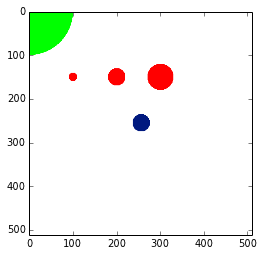
\includegraphics[max size={\textwidth}{\textheight}]{basictests_files/basictests_30_0.png}
\par
\end{center}

\end{InvisibleVerbatim}



\section{Integration with scikit image
}The canvas object publicizes a few image attributes for convienence
for example:

\begin{itemize}
\item
shape
\item
ndim
\item
dtype
\end{itemize}
However, when using ndarray functions, pass the \emph{.image} array
directly.


% Make sure that atleast 4 lines are below the HR
\needspace{4\baselineskip}


\vspace{6pt}
\makebox[0.1\linewidth]{\smaller\hfill\tt\color{nbframe-in-prompt}In\hspace{4pt}{[}28{]}:\hspace{4pt}}\\*
\vspace{-2.65\baselineskip}
\begin{ColorVerbatim}
\vspace{-0.7\baselineskip}
\begin{Verbatim}[commandchars=\\\{\}]
\PY{k+kn}{from} \PY{n+nn}{skimage.filter} \PY{k+kn}{import} \PY{n}{gaussian\PYZus{}filter}\PY{p}{,} \PY{n}{sobel}
\PY{k+kn}{from} \PY{n+nn}{skimage.color} \PY{k+kn}{import} \PY{n}{rgb2gray}

\PY{n}{fig}\PY{p}{,} \PY{p}{(}\PY{n}{ax1}\PY{p}{,} \PY{n}{ax2}\PY{p}{)} \PY{o}{=} \PY{n}{plt}\PY{o}{.}\PY{n}{subplots}\PY{p}{(}\PY{n}{nrows}\PY{o}{=}\PY{l+m+mi}{1}\PY{p}{,} \PY{n}{ncols}\PY{o}{=}\PY{l+m+mi}{2}\PY{p}{,} \PY{n}{figsize}\PY{o}{=}\PY{p}{(}\PY{l+m+mi}{8}\PY{p}{,}\PY{l+m+mi}{8}\PY{p}{)}\PY{p}{)}

\PY{n}{c\PYZus{}filtered} \PY{o}{=} \PY{n}{gaussian\PYZus{}filter}\PY{p}{(}\PY{n}{c}\PY{o}{.}\PY{n}{image}\PY{p}{,} \PY{l+m+mi}{10}\PY{p}{)}
\PY{n}{ax1}\PY{o}{.}\PY{n}{imshow}\PY{p}{(}\PY{n}{c\PYZus{}filtered}\PY{p}{)}
\PY{n}{ax1}\PY{o}{.}\PY{n}{set\PYZus{}title}\PY{p}{(}\PY{l+s}{\PYZsq{}}\PY{l+s}{Guassin blur}\PY{l+s}{\PYZsq{}}\PY{p}{)}

\PY{c}{\PYZsh{} Sobel requires gray image; we convert from rgb}
\PY{n}{c\PYZus{}sobel} \PY{o}{=} \PY{n}{sobel}\PY{p}{(}\PY{n}{rgb2gray}\PY{p}{(}\PY{n}{c\PYZus{}filtered}\PY{p}{)}\PY{p}{)}
\PY{n}{ax2}\PY{o}{.}\PY{n}{imshow}\PY{p}{(}\PY{n}{c\PYZus{}sobel}\PY{p}{,} \PY{n}{plt}\PY{o}{.}\PY{n}{cm}\PY{o}{.}\PY{n}{gray}\PY{p}{)}
\PY{n}{ax2}\PY{o}{.}\PY{n}{set\PYZus{}title}\PY{p}{(}\PY{l+s}{\PYZsq{}}\PY{l+s}{Sobel gradient of blur}\PY{l+s}{\PYZsq{}}\PY{p}{)}\PY{p}{;}
\end{Verbatim}


\vspace{-0.2\baselineskip}

\end{ColorVerbatim}




% If the first block is an image, minipage the image.  Else
% request a certain amount of space for the input text.
\needspace{4\baselineskip}



% Add document contents.

\begin{InvisibleVerbatim}
\vspace{-0.5\baselineskip}
\begin{center}
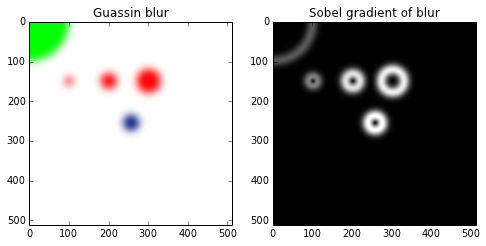
\includegraphics[max size={\textwidth}{\textheight}]{basictests_files/basictests_33_0.png}
\par
\end{center}

\end{InvisibleVerbatim}



\textbf{ONE IMPORTANT CAVEAT:} Since guassian\_filter returns an
array, c\_filtered is no longer a \emph{Canvas}. I may add some
support later to return a \emph{Canvas} object with it's image
attribute overwritten; however, one should keep in mind that the
underlying particles \textbf{are unchanged} by the guassian filter;
only the final ``drawn'' image has been altered. It may therefore
be misleading to add this feature because one would need to remain
aware that these blurry particles are not representative of what is
actually stored by the Canvas. In any case, this is at least a
little more convienent than referring to c.image so often!


% Make sure that atleast 4 lines are below the HR
\needspace{4\baselineskip}


\vspace{6pt}
\makebox[0.1\linewidth]{\smaller\hfill\tt\color{nbframe-in-prompt}In\hspace{4pt}{[}29{]}:\hspace{4pt}}\\*
\vspace{-2.65\baselineskip}
\begin{ColorVerbatim}
\vspace{-0.7\baselineskip}
\begin{Verbatim}[commandchars=\\\{\}]
\PY{n+nb}{type}\PY{p}{(}\PY{n}{c}\PY{p}{)}\PY{p}{,} \PY{n+nb}{type}\PY{p}{(}\PY{n}{c\PYZus{}filtered}\PY{p}{)}
\end{Verbatim}


\vspace{-0.2\baselineskip}

\end{ColorVerbatim}




% If the first block is an image, minipage the image.  Else
% request a certain amount of space for the input text.
\needspace{4\baselineskip}



% Add document contents.

\makebox[0.1\linewidth]{\smaller\hfill\tt\color{nbframe-out-prompt}Out\hspace{4pt}{[}29{]}:\hspace{4pt}}\\*
\vspace{-2.55\baselineskip}\begin{InvisibleVerbatim}
\vspace{-0.5\baselineskip}
\begin{alltt}(pyparty.tools.canvas.Canvas, numpy.ndarray)\end{alltt}

\end{InvisibleVerbatim}



\section{Multiplots with matplotlib
}Canvas has a \emph{.show()} method that wraps imshow. This has been
called already above to produce the output images. \emph{.show()}
also optionally accepts AxesSubPlot objects from matplotlib (these
are returned by plt.subplots() ). Thus, it's easy to create
multiple plots


% Make sure that atleast 4 lines are below the HR
\needspace{4\baselineskip}


\vspace{6pt}
\makebox[0.1\linewidth]{\smaller\hfill\tt\color{nbframe-in-prompt}In\hspace{4pt}{[}30{]}:\hspace{4pt}}\\*
\vspace{-2.65\baselineskip}
\begin{ColorVerbatim}
\vspace{-0.7\baselineskip}
\begin{Verbatim}[commandchars=\\\{\}]
\PY{n}{fig}\PY{p}{,} \PY{p}{(}\PY{n}{ax1}\PY{p}{,} \PY{n}{ax2}\PY{p}{,} \PY{n}{ax3}\PY{p}{)} \PY{o}{=} \PY{n}{plt}\PY{o}{.}\PY{n}{subplots}\PY{p}{(}\PY{n}{nrows}\PY{o}{=}\PY{l+m+mi}{1}\PY{p}{,} \PY{n}{ncols}\PY{o}{=}\PY{l+m+mi}{3}\PY{p}{,} \PY{n}{figsize} \PY{o}{=} \PY{p}{(}\PY{l+m+mi}{10}\PY{p}{,}\PY{l+m+mi}{10}\PY{p}{)}\PY{p}{)}

\PY{n}{ax1}\PY{o}{.}\PY{n}{set\PYZus{}title}\PY{p}{(}\PY{l+s}{\PYZsq{}}\PY{l+s}{ax1}\PY{l+s}{\PYZsq{}}\PY{p}{)}
\PY{n}{c}\PY{o}{.}\PY{n}{show}\PY{p}{(}\PY{n}{ax1}\PY{p}{)}

\PY{c}{\PYZsh{}Add a particle}
\PY{n}{c}\PY{o}{.}\PY{n}{add}\PY{p}{(}\PY{l+s}{\PYZsq{}}\PY{l+s}{circle}\PY{l+s}{\PYZsq{}}\PY{p}{,} \PY{n}{name}\PY{o}{=}\PY{l+s}{\PYZsq{}}\PY{l+s}{cyanparticle}\PY{l+s}{\PYZsq{}}\PY{p}{,} \PY{n}{radius}\PY{o}{=}\PY{l+m+mi}{20}\PY{p}{,} \PY{n}{center}\PY{o}{=}\PY{p}{(}\PY{l+m+mi}{400}\PY{p}{,}\PY{l+m+mi}{100}\PY{p}{)}\PY{p}{,} \PY{n}{color}\PY{o}{=}\PY{p}{(}\PY{l+m+mi}{0}\PY{p}{,}\PY{l+m+mi}{1}\PY{p}{,}\PY{l+m+mi}{1}\PY{p}{)}\PY{p}{)}

\PY{n}{ax2}\PY{o}{.}\PY{n}{set\PYZus{}title}\PY{p}{(}\PY{l+s}{\PYZsq{}}\PY{l+s}{ax2 (extra cyan particle)}\PY{l+s}{\PYZsq{}}\PY{p}{)}
\PY{n}{c}\PY{o}{.}\PY{n}{show}\PY{p}{(}\PY{n}{ax2}\PY{p}{)}

\PY{c}{\PYZsh{}Reuse an old background for plot, then clear it}
\PY{n}{ax3}\PY{o}{.}\PY{n}{set\PYZus{}title}\PY{p}{(}\PY{l+s}{\PYZsq{}}\PY{l+s}{ax3 (moon background)}\PY{l+s}{\PYZsq{}}\PY{p}{)}
\PY{n}{c}\PY{o}{.}\PY{n}{background} \PY{o}{=} \PY{n}{moon}\PY{p}{(}\PY{p}{)}
\PY{n}{c}\PY{o}{.}\PY{n}{show}\PY{p}{(}\PY{n}{ax3}\PY{p}{)}\PY{p}{;}
\end{Verbatim}


\vspace{-0.2\baselineskip}

\end{ColorVerbatim}




% If the first block is an image, minipage the image.  Else
% request a certain amount of space for the input text.
\needspace{4\baselineskip}



% Add document contents.

\begin{InvisibleVerbatim}
\vspace{-0.5\baselineskip}
\begin{alltt}12-12 22:16:10 WARNING  pyparty.tools.canvas:  background color has
been converted (from grayscale to RGB)
\end{alltt}

\end{InvisibleVerbatim}

\begin{InvisibleVerbatim}
\vspace{-0.5\baselineskip}
\begin{center}
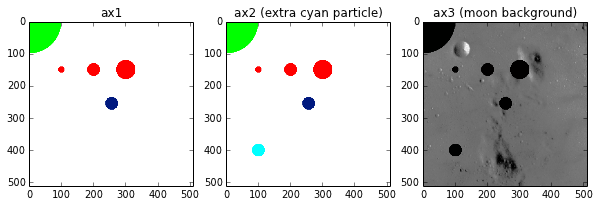
\includegraphics[max size={\textwidth}{\textheight}]{basictests_files/basictests_38_1.png}
\par
\end{center}

\end{InvisibleVerbatim}



\subsection{Clearing the particles/objects
}The important methods are:

\begin{itemize}
\item
remove(index or name) : Removes a single particle from canvas \#NOT
YET IMPLELMENTED
\item
clear\_background() : Removes all particles from the canvas
\item
clear\_particles() : Resets the background image to the default
\item
clear\_canvas() : Removes all particles \textbf{and} resets the
background
\end{itemize}
First, let's clear out the cyan particle that was just added. Since
we named it ``cyanparticle'', this it is easy to access


% Make sure that atleast 4 lines are below the HR
\needspace{4\baselineskip}


\vspace{6pt}
\makebox[0.1\linewidth]{\smaller\hfill\tt\color{nbframe-in-prompt}In\hspace{4pt}{[}31{]}:\hspace{4pt}}\\*
\vspace{-2.65\baselineskip}
\begin{ColorVerbatim}
\vspace{-0.7\baselineskip}
\begin{Verbatim}[commandchars=\\\{\}]
\PY{k}{print} \PY{l+s}{\PYZsq{}}\PY{l+s}{particles \PYZhy{}\PYZhy{}\PYZhy{}\PYZgt{}}\PY{l+s}{\PYZsq{}}\PY{p}{,}\PY{n}{c}\PY{o}{.}\PY{n}{particles}
\end{Verbatim}


\vspace{-0.2\baselineskip}

\end{ColorVerbatim}




% If the first block is an image, minipage the image.  Else
% request a certain amount of space for the input text.
\needspace{4\baselineskip}



% Add document contents.

\begin{InvisibleVerbatim}
\vspace{-0.5\baselineskip}
\begin{alltt}particles ---> ['centered\_particle', 'circle\_4', 'circle\_3',
'cyanparticle', 'circle\_5', 'edge\_particle', 'outside\_particle']
\end{alltt}

\end{InvisibleVerbatim}





% Make sure that atleast 4 lines are below the HR
\needspace{4\baselineskip}


\vspace{6pt}
\makebox[0.1\linewidth]{\smaller\hfill\tt\color{nbframe-in-prompt}In\hspace{4pt}{[}32{]}:\hspace{4pt}}\\*
\vspace{-2.65\baselineskip}
\begin{ColorVerbatim}
\vspace{-0.7\baselineskip}
\begin{Verbatim}[commandchars=\\\{\}]
\PY{n}{c}\PY{o}{.}\PY{n}{clear\PYZus{}canvas}\PY{p}{(}\PY{p}{)}
\PY{k}{print} \PY{l+s}{\PYZsq{}}\PY{l+s}{particles \PYZhy{}\PYZhy{}\PYZhy{}\PYZgt{}}\PY{l+s}{\PYZsq{}}\PY{p}{,} \PY{n}{c}\PY{o}{.}\PY{n}{particles}
\PY{n}{c}\PY{o}{.}\PY{n}{show}\PY{p}{(}\PY{p}{)}\PY{p}{;}
\end{Verbatim}


\vspace{-0.2\baselineskip}

\end{ColorVerbatim}




% If the first block is an image, minipage the image.  Else
% request a certain amount of space for the input text.
\needspace{4\baselineskip}



% Add document contents.

\begin{InvisibleVerbatim}
\vspace{-0.5\baselineskip}
\begin{alltt}particles ---> []
\end{alltt}

\end{InvisibleVerbatim}

\begin{InvisibleVerbatim}
\vspace{-0.5\baselineskip}
\begin{center}
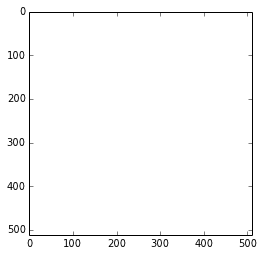
\includegraphics[max size={\textwidth}{\textheight}]{basictests_files/basictests_42_1.png}
\par
\end{center}

\end{InvisibleVerbatim}



\section{Indexing/Slicing
}


\renewcommand{\indexname}{Index}
\printindex

% End of document
\end{document}

